
\documentclass[11pt,a4paper]{article}

\usepackage{fouriernc}
\usepackage[utf8]{inputenc}   % Je kunt gewóón accenten typen, als je wilt
\usepackage[T1]{fontenc}      % Nodig om de accenten ook ín de pdf te krijgen
\usepackage[english]{babel}
\usepackage{graphicx}
\usepackage{amssymb}
\usepackage{amsmath}          % Voor extra ondersteuning bij vergelijkingen (zie documentatie)
\usepackage{natbib}           % Voor auteur-jaar citatie.
\usepackage{a4wide}           % Past marges aan voor A4.
\usepackage[small]{caption}   % Voor bijschriften met een iets kleinere lettergrootte dan de hoofdtekst.
\usepackage{url}              % Voor het beter weergeven van url's (lang, of met speciale tekens)
\usepackage{booktabs}         % Voor professionele tabellen
\usepackage[output-decimal-marker={,},list-final-separator={ en }]{siunitx}          % Voor het typesetten en uitlijnen van getallen en eenheden, zie documentatie
\usepackage[pdfusetitle]{hyperref}  % Voor handige links in je PDF. B.v. urls, referenties, etc.
\usepackage{listings}
\linespread{1.3}              % Iets grotere regelafstand: fijn voor degene die het nakijkt.
\usepackage{mathrsfs,amsmath} 
% \renewcommand{\arraystretch}{1.5}   % Om rijen in tabellen wat ruimer rond de tekst te maken.
\usepackage{tabularx}
\usepackage{rotating}
\usepackage{pdflscape}
\usepackage[utf8]{inputenc}
\graphicspath{{../data}} %Setting the graphicspath

\title{CP II; Ising Model}
\author{Brandon Parfimczyk, Kien Do \& Mario van Rooij }
\date{16-2-2020}

\begin{document}

\maketitle

\tableofcontents
\newpage

\section{Manual}

For the main program one needs to run the following scripts:
\begin{enumerate}
    \item ‘make ising-sim’ 
    \item ‘make auto’
    \item ‘gen\_data.sh’ (get history of observables)
    \item ‘gen\_data2.sh’ (get autocorrelation data)
    \item ‘gen\_plot\_M.sh’ (get some statistics and with this one can plot magnetization - beta) 
    \item 'all\_plot.sh' (generates all the plots)
    
        \subitem Then there are the scripts to generate the individual plots when desired:
        \subitem 'data\_ac\_energy.plt' (generates autocorrelation plots using the energy)
        \subitem 'data\_ac\_magnet.plt' (generates autocorrelation plots using magnetization)
        \subitem 'data\_M-T.plt' (plot for magnetization as a function of temperature with different $B$)
        \subitem 'data\_energy.plt' (plot for the energies of the system with different parameters)
        \subitem 'data\_energy\_f300.plt'(First 300 energy values of system with different parameters)
        \subitem 'data\_magnet.plt'(plot for the magnetization of the system with different parameters)
        \subitem 'data\_magnet\_f300.plt' (First 300 magnetization values of system with different parameters)

    \item Main program
        \subitem There are 5 parameters that can be given to the main program:
        \subitem $\beta$ (given as b in the parameters), the inverse temperature
        \subitem $B$, the magnetic field
        \subitem s, the seed
        \subitem D, the amount of dimensions of the system
        \subitem N, the amount of points per dimension
        \subitem Example: Run the make 'ising-sim' file and run the executable ising-sim file (ising-sim in executables) with the parameters: 
    ising-sim -N 1000 -D 5 -b 0.4 (the rest of the parameters can be left to the standard parameters found in gen\_data.sh) 
\end{enumerate}

\section{Planning}

The planning in this project was the following:

28.01 - All team members will have read the document on the Ising model.

29.01 - Required code and tests are listed and role distribution is made. 

04.02 - Finished code for Monte-Carlo, energy calculation and spin configurations generator.

06.02 - Implemented $ising-sim.c$

12.02 - Finished autocorrelation code

16.02 - Finalized project

\section{Notes from lecture}

Start from any initial condition. $s_0 \xrightarrow{mc step} s_1 \xrightarrow{mc step} s_2  \xrightarrow{mc step}$ etc.

$H_{0}, H_1 , H_2$ Monte Carlo history of the energy. Make a plot H vs MC time. Discrete fluctuations. Influence from initial conditions is called thermalization. Throw away part of thermalization. 

\begin{equation}
    <H> \approx \frac{1}{N-n_T}\sum_{n = n_T}^{N-1} H_n,
\end{equation}

where $N$ is the number of steps, $n_T$ is the amount of steps until thermalization and $H_n$ is the energy of the system in the n-th step.

\subsection{Error in the observables}


Mean of Monte-Carlo chain: 
\begin{equation}
    \hat{H} = \frac{1}{N} \sum_{n = 0}^{N-1 } H_n
\end{equation}

Variance:

\begin{equation}
    \sigma_{H}^2 = \frac{1}{N} \sum_{n = 0}^{N-1 } (H_n - \hat{H})^2
\end{equation}

Standard deviation:

\begin{equation}
    \sigma_{H} = \sqrt{\frac{1}{N} \sum_{n = 0}^{N-1 } (H_n - \hat{H})^2}
\end{equation}

Histogram as a function of energy. We need something different from the standard deviation, because it does not change with $N$. Central limit theorem. If the configurations are independent the error of the estimate of the average is equal to:

\begin{equation}
   \sigma_{\Bar{H}} = \frac{\sigma_H}{\sqrt{N-1}}
\end{equation}

But the configurations are not independent. The Markov-Chains will have auto-correlation. Make an estimation for the amount of steps for 2 configurations to be independent. This amount of steps is called the autocorrelation time.

For non-indepedent configurations one looks at: $\tau_{AC}$ (Autocorrelation time)

\begin{equation}
N_{eff} = \frac{N}{2 \tau_{AC}}
\end{equation}

\section{Code recycling}

The project can rely on some code of the previous project. This includes the codes for generating indices from coordinates and vice versa and parts of code for the Laplacian, since this already uses the nearest neighbours. The recycled functions are:
\begin{enumerate}
    \item ind2coord()
    \item coord2ind()
    \item nn\_neighbour()
    \item nn\_create()
\end{enumerate}

\section{Modules}

functions.c : Contains code for configuring the system, calculations for various parameters of the system and the main algoritms. This includes the average energy, magnetization and the monte\_carlo algoritm.

geometry.c : Code for calculations done with the geometry. Nearest neighbour array calculation, coordinate to index and index to coordinate.

main program: The setup for the main program will be as follows: First one runs the program with given variables and some plot is shown to decide by eye what the amount of steps is where thermalization has been reached. After that, the parameters are calculated again.

Ising-sim.c: Program that runs the simulation. Parameters are changed in this code. There are options for magnetic field ($B$), dimensions ($D$), number of lattice points per dimension ($N$) and temperature ($b$).

\section{Testing}

\subsection{NN-testing}

The nearest neighbour function can be tested by looping through all points, and checking for every point that the nearest neighbour array contains coordinates that differ by only 1, or -1 in all directions with the special condition at the boundaries.

\subsection{Energy test}

Tests if the energy calculator is the same as an initial analytically known energy for a system configuration.

One anomaly that occurred in the test for the energy was the difference between calulating the energy by summing up the spin-magnetic interaction per spin-site and the multiplication of all the spins summed multiplied by the magnetic field:

\begin{equation}
E_{B} = \sum_{x} B  * s(x) 
\end{equation}
\label{sum_1}
\begin{equation}
E_{B} = B \sum_{x} s(x) 
\label{sum_2}
\end{equation}

When the test for the energy is ran the difference in the values can be seen. The reason for this is that the amount of calculations in formula \ref{sum_1} requires more calculations, which makes the error accumulate.

\subsection{Monte carlo}

Since this algoritm relies on a stochastic process, it is not possible to test this algoritm. The code could only be compared to other groups. One test that can be done however, is starting with different initial configurations and seeing if the configurations converge to the same equilibrium. This is done in the monte-carlo test. The test reveals that all forget their initial configuration after some time, which is good since this is the intrinsic property of markov chain and they stabilize around a range of certain values. The values printed last in the table are inside the variances and thus fulfill the test.

\section{Codes to be designed}

Hamiltonian:

Initial energy calculation. For the rest of the configuration a sum can be used instead of looping over the whole lattice.

Monte carlo:

Code that renders what the next step in the markov-chain looks like.

2-point correlation function.

\section{Optimization}

In order to calculate the initial energy of the system, one only needs the array of the forward neighbours, but since this calculation is done only once, it is not worth it to generate this array.

Furthermore the difference in energy per markov-chain can be calculated by the difference with the previous one. This way one does not have to loop over the whole array every $s$ to get the energy for this configuration.

There is also a optimization possibility in [ geometry.c : nn\_create() ] by allocating one continuous block of memory (one call to malloc) and then assign the pointers to different points inside the array. In our code it's implemented by calling malloc for each pointer. This can lead to a memory access penalty because in our usage the nn array gets looked up very often and the adjacent memory location could be accessed faster.

\section{Result}

The following plots were found. All the systems were done with $N$ = 100 and $D$ = 2. All the data is from one configuration.

\begin{sidewaysfigure}
\centering
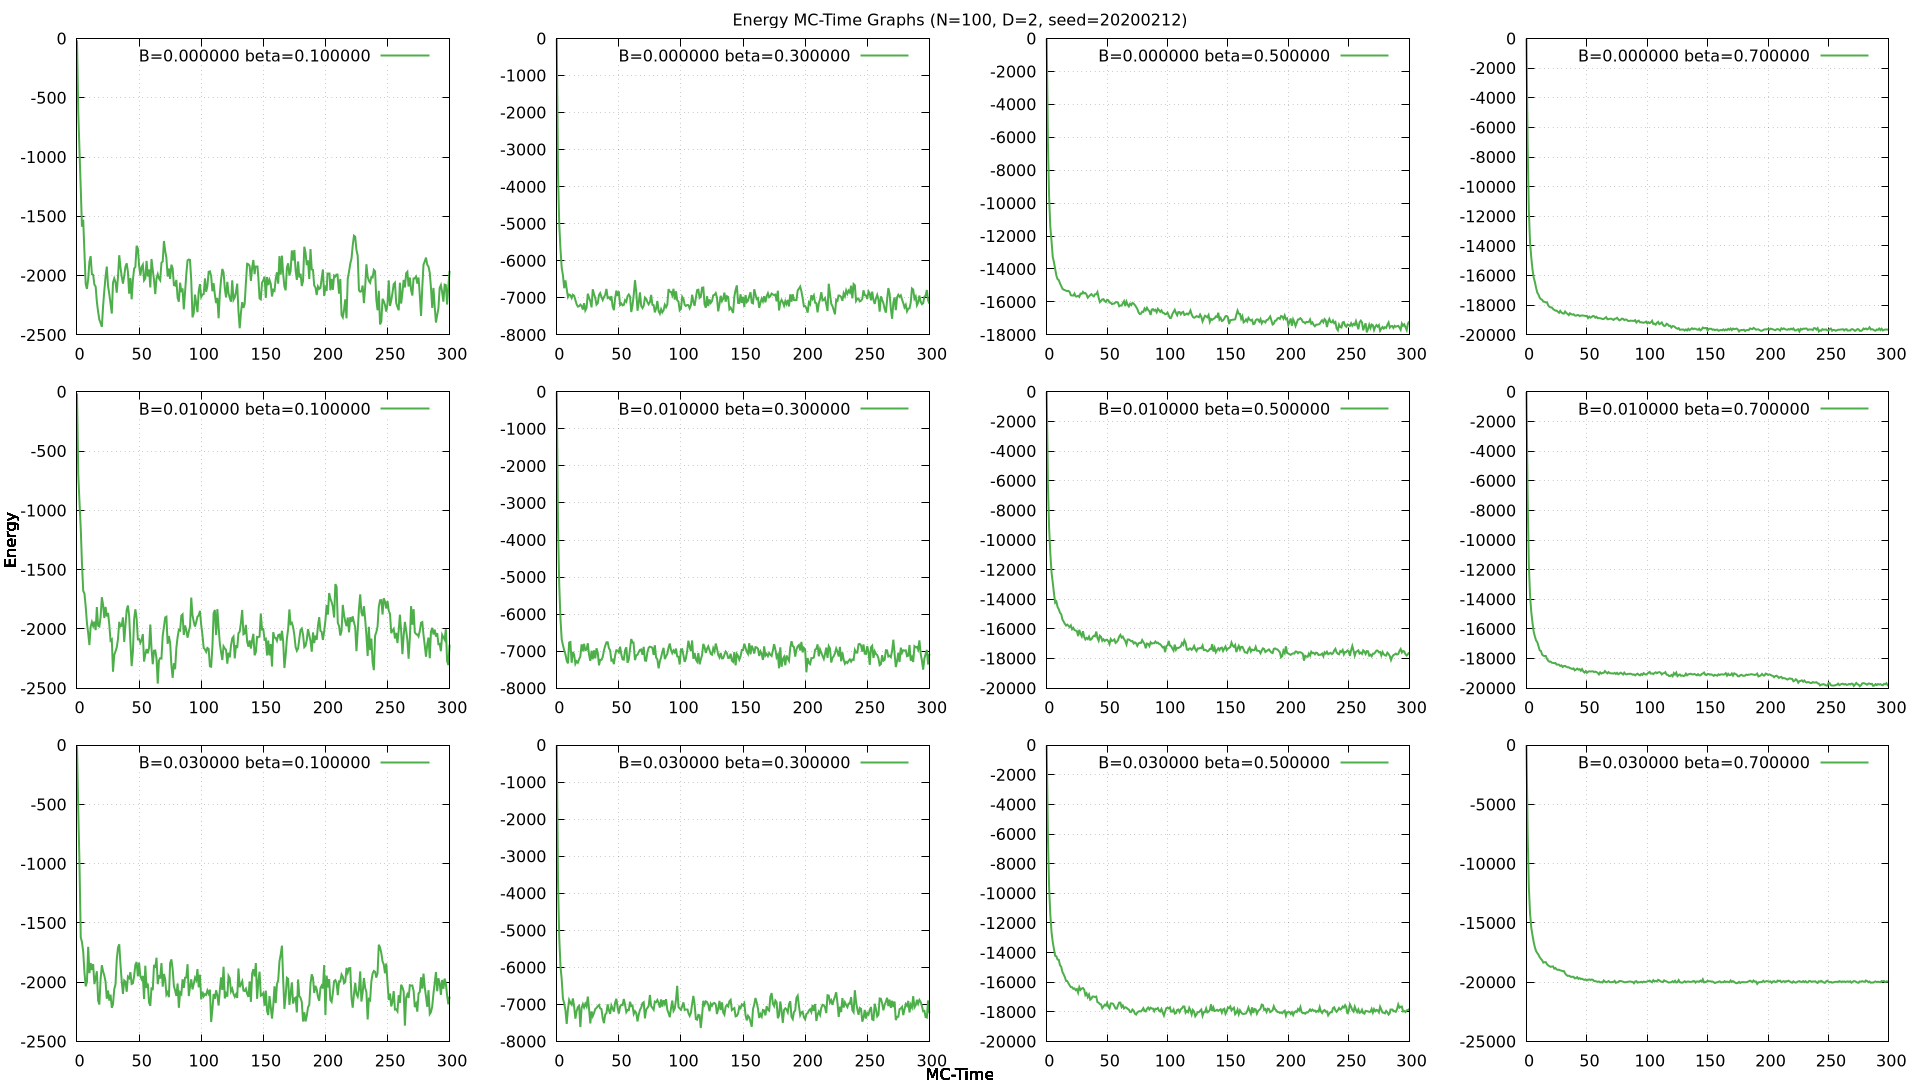
\includegraphics[scale=0.35]{all_energy_f300.png}
\caption{First 300 energies of configurations with the different parameters. Here it can be seen that the system needs multiple steps to stabilize. Because it is a stochastic process, one can not say with 100\% certainty that this is the real stabile point in phase space.}.
\label{fig:foo}
\end{sidewaysfigure}


\begin{sidewaysfigure}
\centering
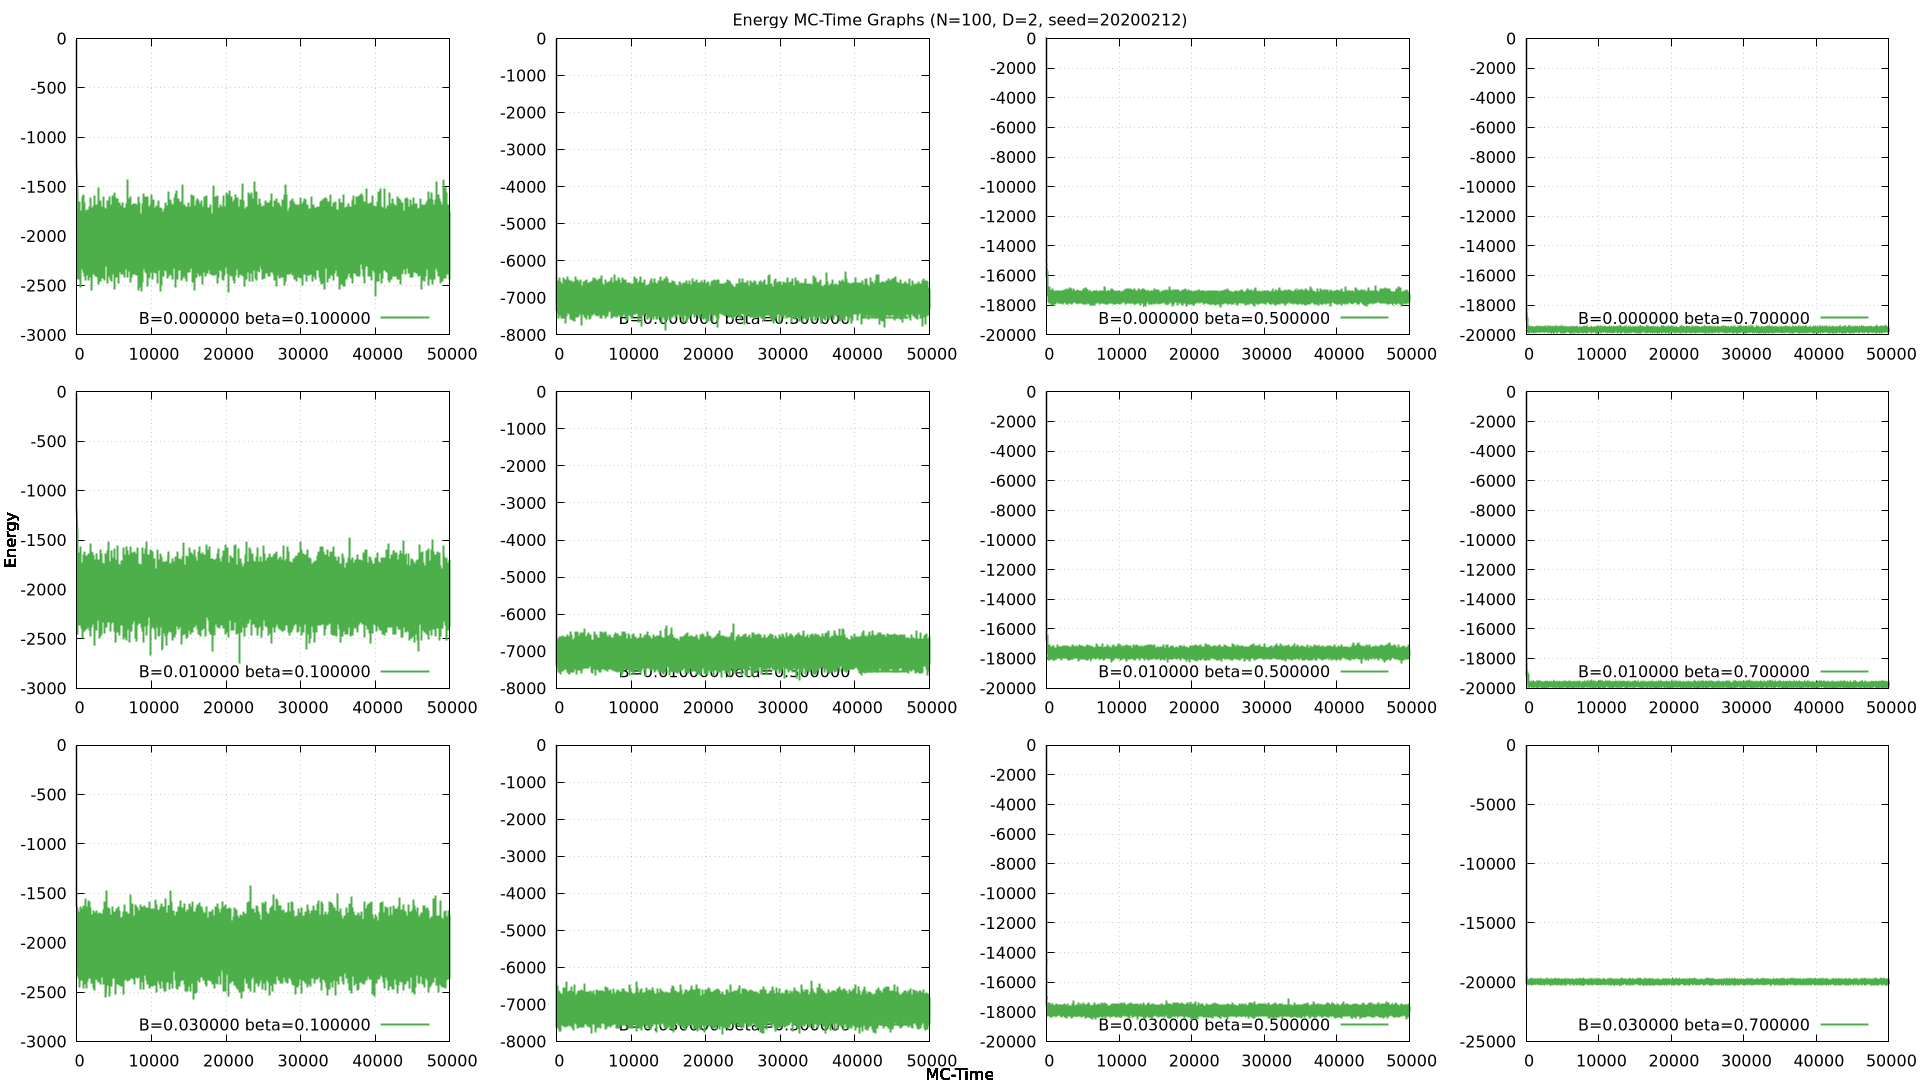
\includegraphics[scale=0.35]{all_energy.png}
\caption{Energies of configurations with the different parameters. Left to right: increasing $\beta$ = \{0.1, 0.3, 0.5, 0.7 \}(lower temperature), top to bottom: increasing $B$ = \{0, 0.01 , 0.03 \}.}.
\label{fig:foo2}
\end{sidewaysfigure}
\begin{sidewaysfigure}
\centering
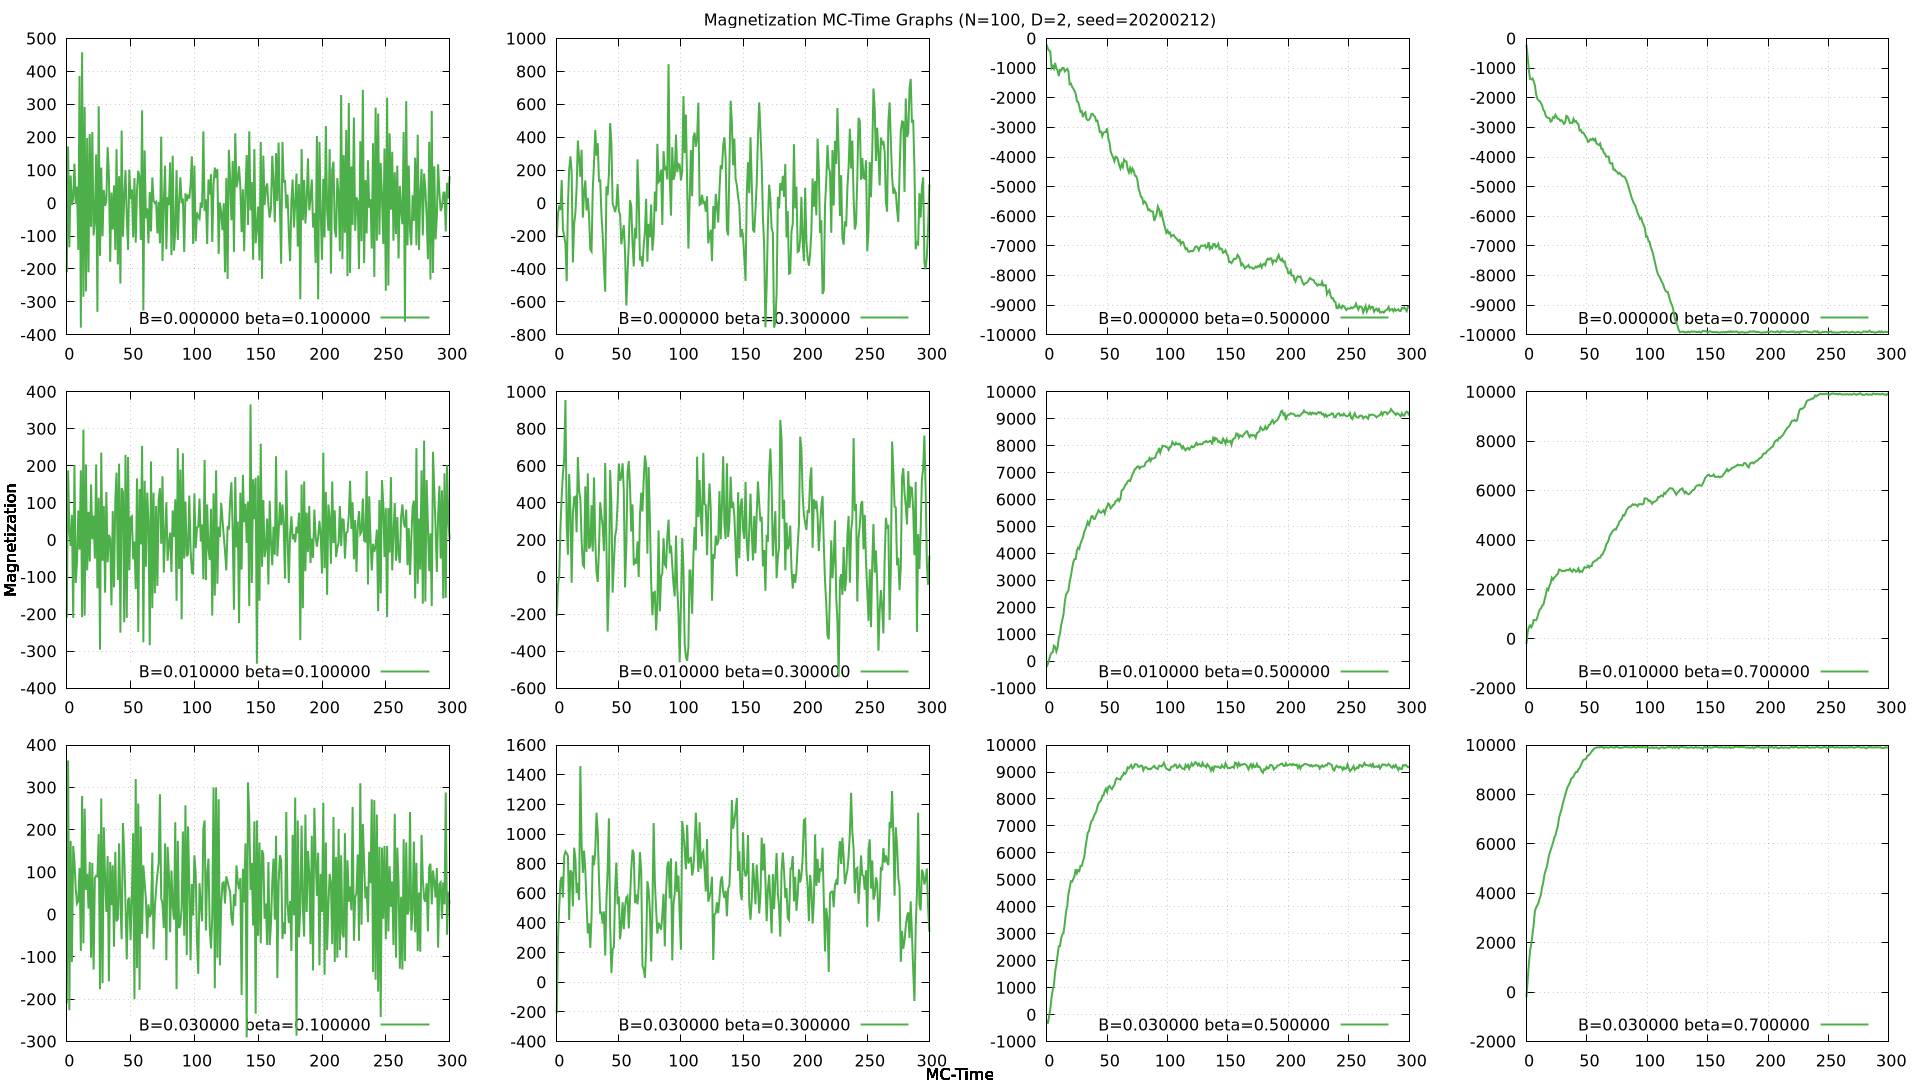
\includegraphics[scale=0.35]{all_magnet_f300.png}
\caption{First 300 magnetizations of configurations with the different parameters. Here it can be seen that the system needs multiple steps to stabilize. Because it is a stochastic process, one can not say with 100\% certainty that this is the real stabile point in phase space.}
\label{fig:foo}
\end{sidewaysfigure}

\begin{sidewaysfigure}
\centering
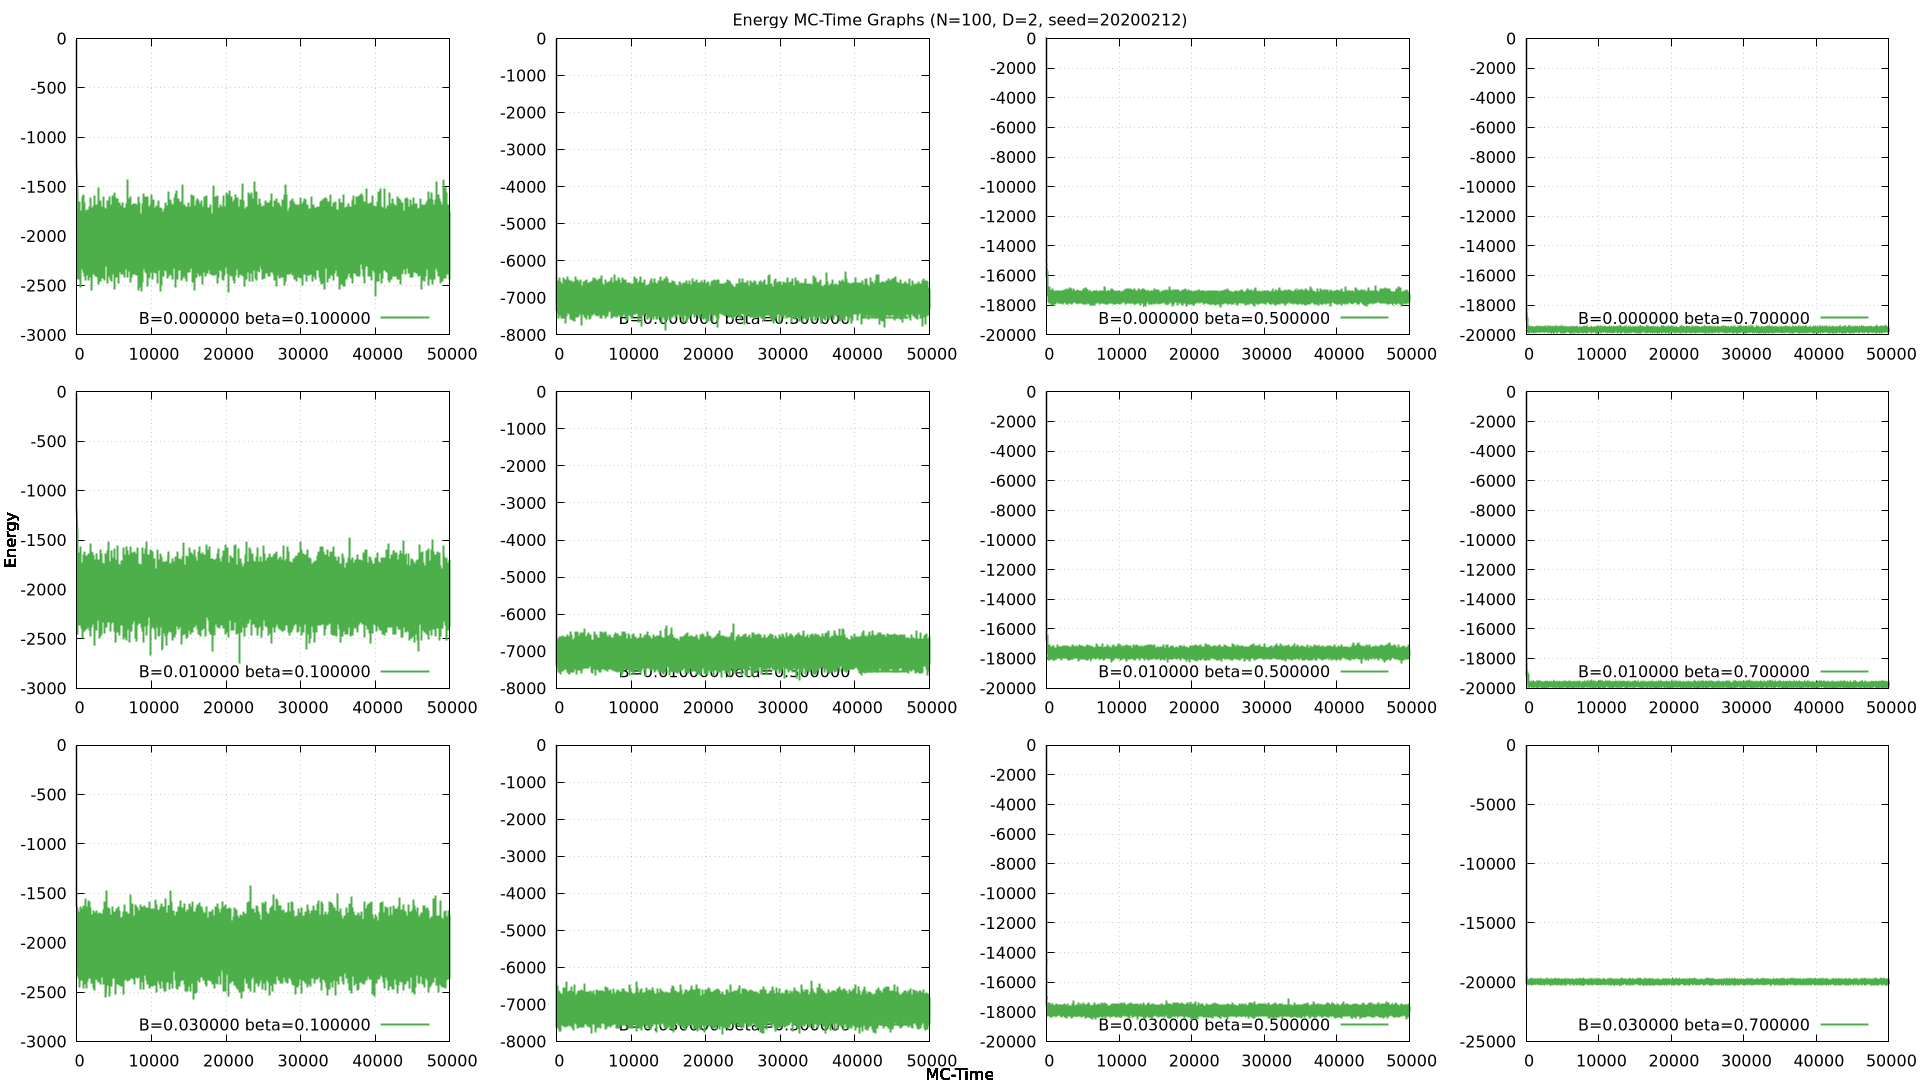
\includegraphics[scale=0.35]{all_energy.png}
\caption{Energies of configurations with the different parameters. Left to right: increasing $\beta$ = \{0.1, 0.3, 0.5, 0.7 \}(lower temperature), top to bottom: increasing $B$ = \{0, 0.01 , 0.03 \}.}.
\label{fig:foo2}
\end{sidewaysfigure}

\begin{sidewaysfigure}
\centering
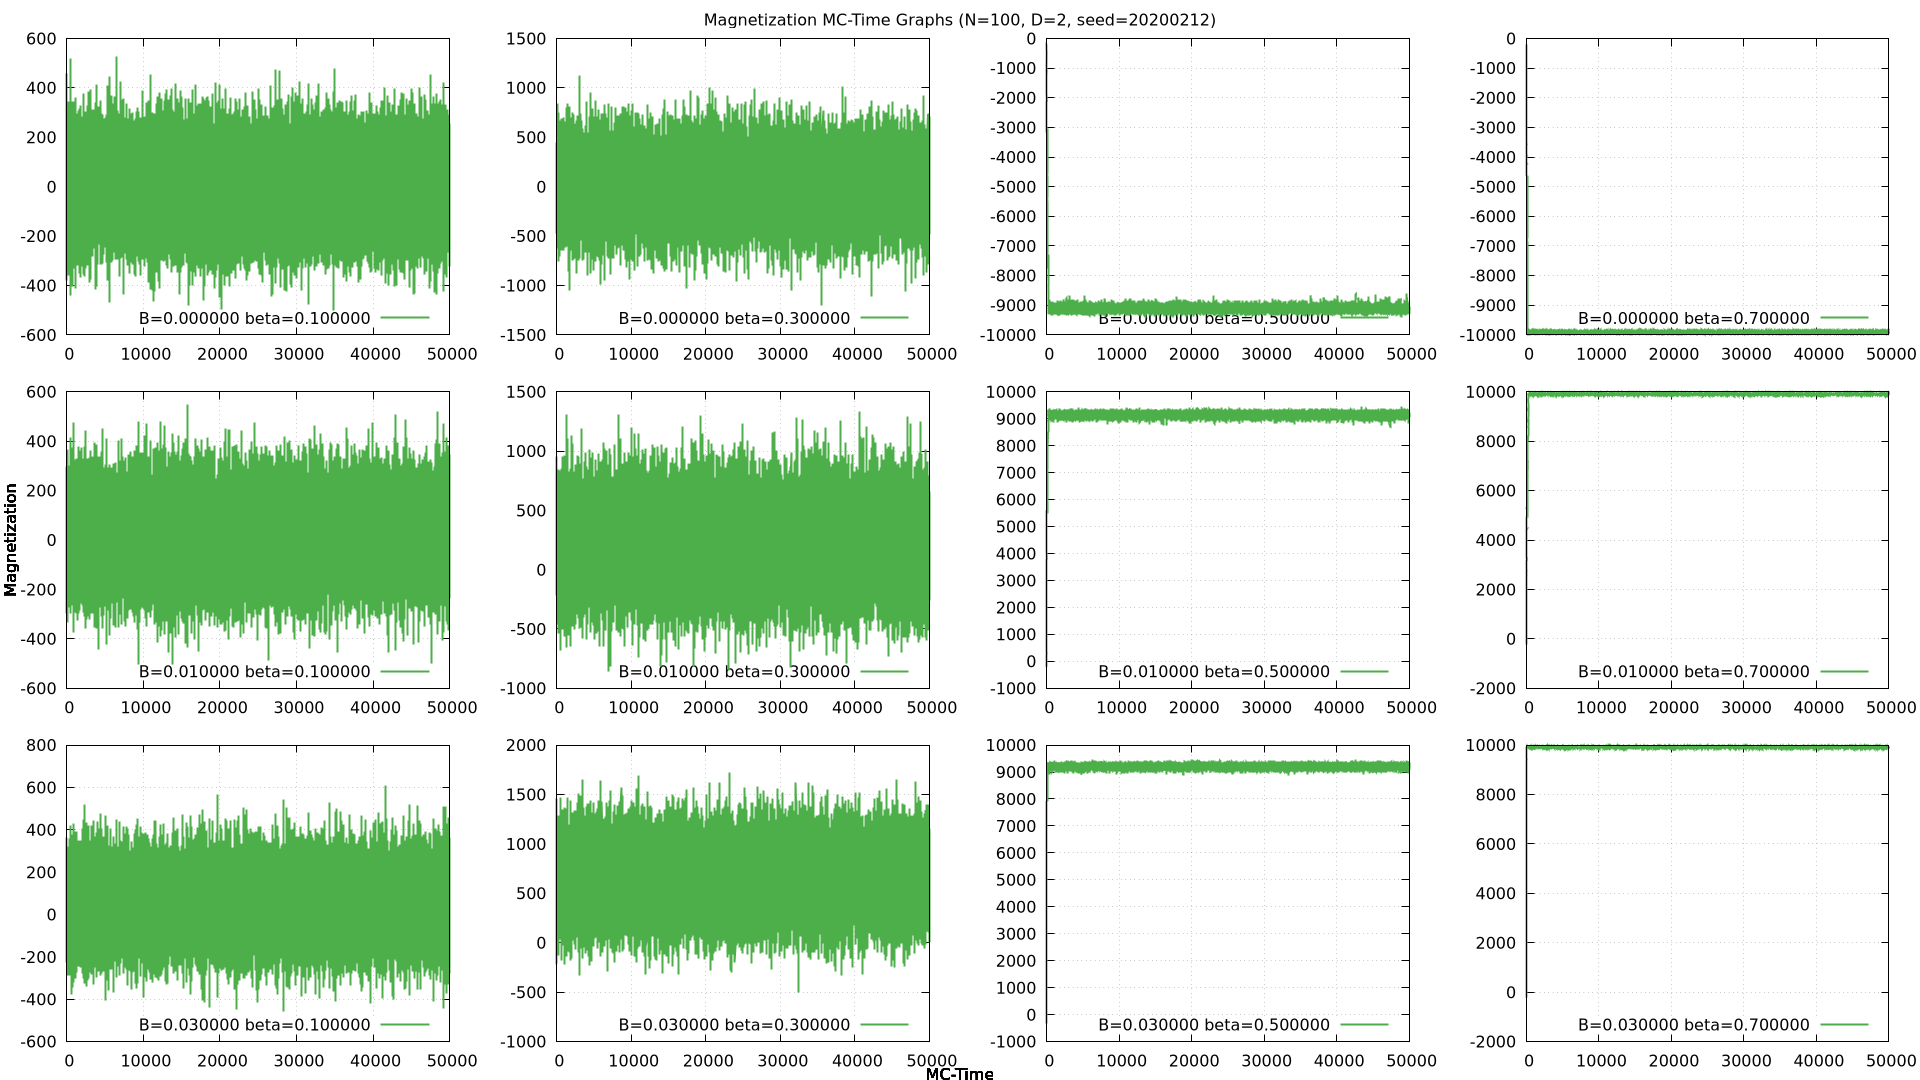
\includegraphics[scale=0.35]{all_magnet.png}
\caption{Magnetization of the system with different parameters. Left to right: increasing $\beta$ = \{0.1, 0.3, 0.5, 0.7 \}(lower temperature), top to bottom: increasing $B$ = \{0, 0.01 , 0.03 \}. The addition of a magnetic field is the most interesting in the second region, where it magnetizes the material.}
\label{fig:foo3}
\end{sidewaysfigure}
One can deduce that there is a phase transition at some combinations of values for $\beta$ and $B$.

\subsection{Physical analysis}

One system that can be simulated is a ferromagnetic system at low temperature. This system can be seen in the lower right in figure \ref{fig:foo3}. Here one can see the physical behaviour of a magnet. A ferromagnet will stay magnetized indefinetly when the temperature is low enough. One can also see that the average magnetization decreases as a function of the temperature (moving to the left in figure \ref{fig:foo3}), the system has more tendency to flip the spins, because the energy loss of the system is smaller. This demagnetization can also be seen in real systems when heating up ferromagnets.

In figure \ref{fig:foo} one can see that the amount of steps to thermalization for system with a higher temperature is lower. This means that the system moves towards equilibrium faster. This makes intuitive sense, because systems generally move towards an equilibrium more quickly at high temperatures (a drop of ink falling into water or chemical reactions).

One can see that the magnetic field adds no significance in the third and fourth temperature regime, since all the spins were already unlikely to be non-parallel, but in the first and second regime, one can see the competing effects of the spin- and magnetic energy effects.

Other observations of possible interesting physical phenomena is the metastable state for low temperature in figure \ref{fig:foo}. Also, the for the value $B = 0.03$ and $\beta = 0.1$ the autocorrelation function flips every time. This is because at this high temperature the magnetization is erased. For $\beta = 0.3$ this is not the case anymore.

In figure \ref{fig:foo70} one can also see that as $\beta$ gets smaller the magnetization approaches zero. This makes, as with the ferromagnetic, physical sense, since a low $\beta$ corresponds to a higher temperature. At some point the ferromagnet reaches the Curie temperature, where the order in the lattice is destroyed and the magnet loses its magnetization.

Another thing that happens in smaller systems is the flip of the magnetization. In real life this phenomenon can not be observed, since the systems are too big and the probability of the magnetization flip is negatively correlated to the volume of the system.

\subsection{Anomalies}

A weird phenomenon can be seen in figure \ref{fig:foo}. Here the thermalization of the system is higher for the lower $\beta$, which would mean the thermalization takes longer for a system a higher temperature. The cause of this may be one of stochastic origin. 




\section{Numerical analysis}

Choice of auto correlation time (on $B$ = 0.0, $\beta$ = 0.05).

One can see in figure \ref{fig:foo32} what the autocorrelation function looks like. It falls off exponentially, which is physically reasonable. After that, it approaches 0 quickly compared to the configuration number. After this it fluctuates with a magnitude of around $10E-2$. This time will simply be called the "stationary time", which is in the range ~100-30.000 of the markov chain.

In figure \ref{fig:foo32} one can see that, with increasing timesteps, the function starts to fluctuate stronger due to the finiteness of data set. Therefore one needs to cut it off at some point to get reasonable data to fit the function and thus finding out the autocorrelation time.

The "point" at which this happened was found using "autocorrelation.c". In figure \ref{fig:foo70} it is visible that this time fluctuates. In the interval [0,2000] the mean value is around 2, before the mean value starts moving. Even the mean value seems to be fluctuating between -4 and 4 (but negative numbers make no sense for time).

The suspected reason for this is that the used distribution for the random number is not i.i.d. This means that the distributions are skewed at different times. Since many small numbers are added togheter, the above described behaviour is obtained.

\subsection{Comparison of auto correlation time methods}

In general, the integrated autocorrelation time in our choice of tail cutting seems to be bigger than with the fitting method. This can be seen by comparing the 2 columns in table \ref{tabel} ($1/t_{ac_E}$ and $1/t_{ac_M}$) with figures \ref{fig:foo70} and \ref{fig:foo71}.

\subsection{Note on autocorr.c}

Although one should find out this "stationary time" individually for all set of parameters, it is practically very hard to get a good approximation on it. As we checked manually, we thus decided out of practical reasons to only use one one stationary time, called "cut" in our autocorr.c.One can extend this by adding another option in the command handling, similar to what we did for the thermalization time. 
  


\begin{sidewaysfigure}
\centering
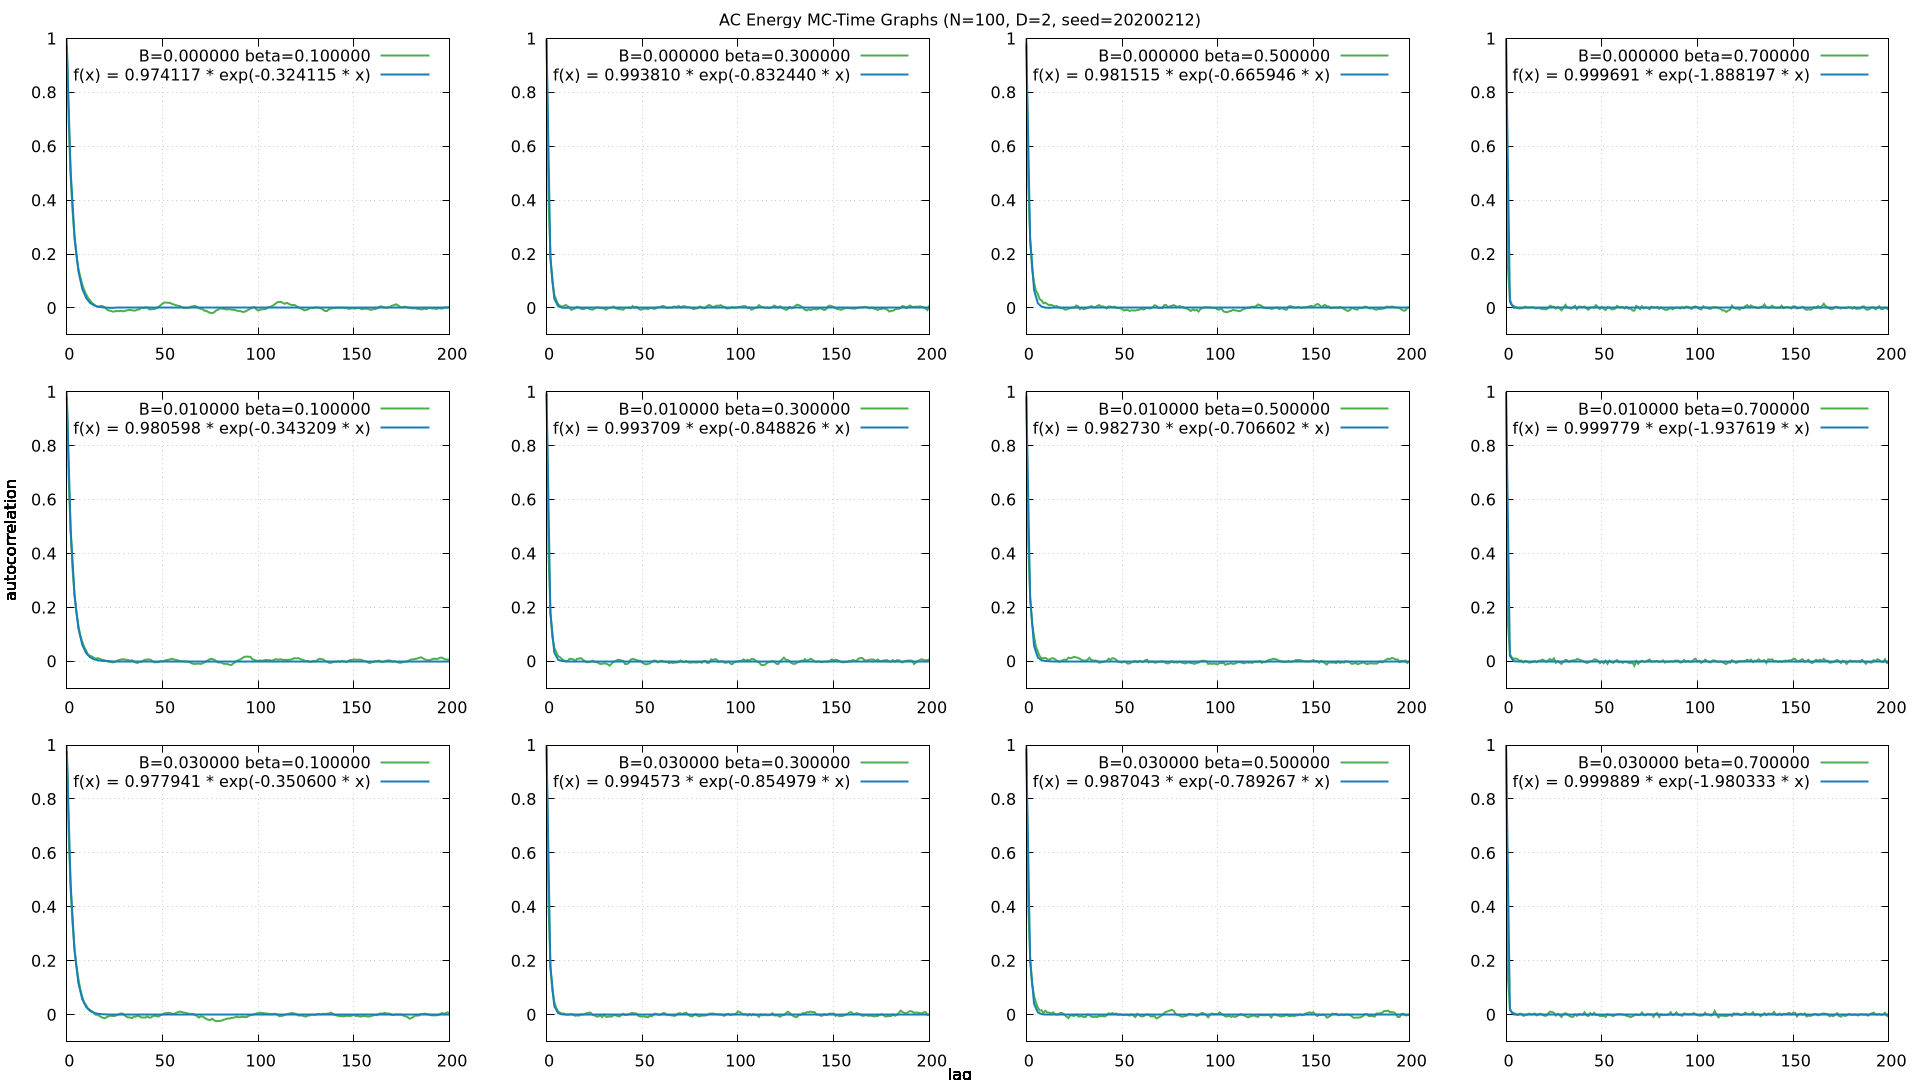
\includegraphics[scale=0.50]{all_ac_energy.png}
\caption{Autocorrelation plotted against the mc-step using the energy}.
\label{fig:foo70}
\end{sidewaysfigure}

\begin{sidewaysfigure}
\centering
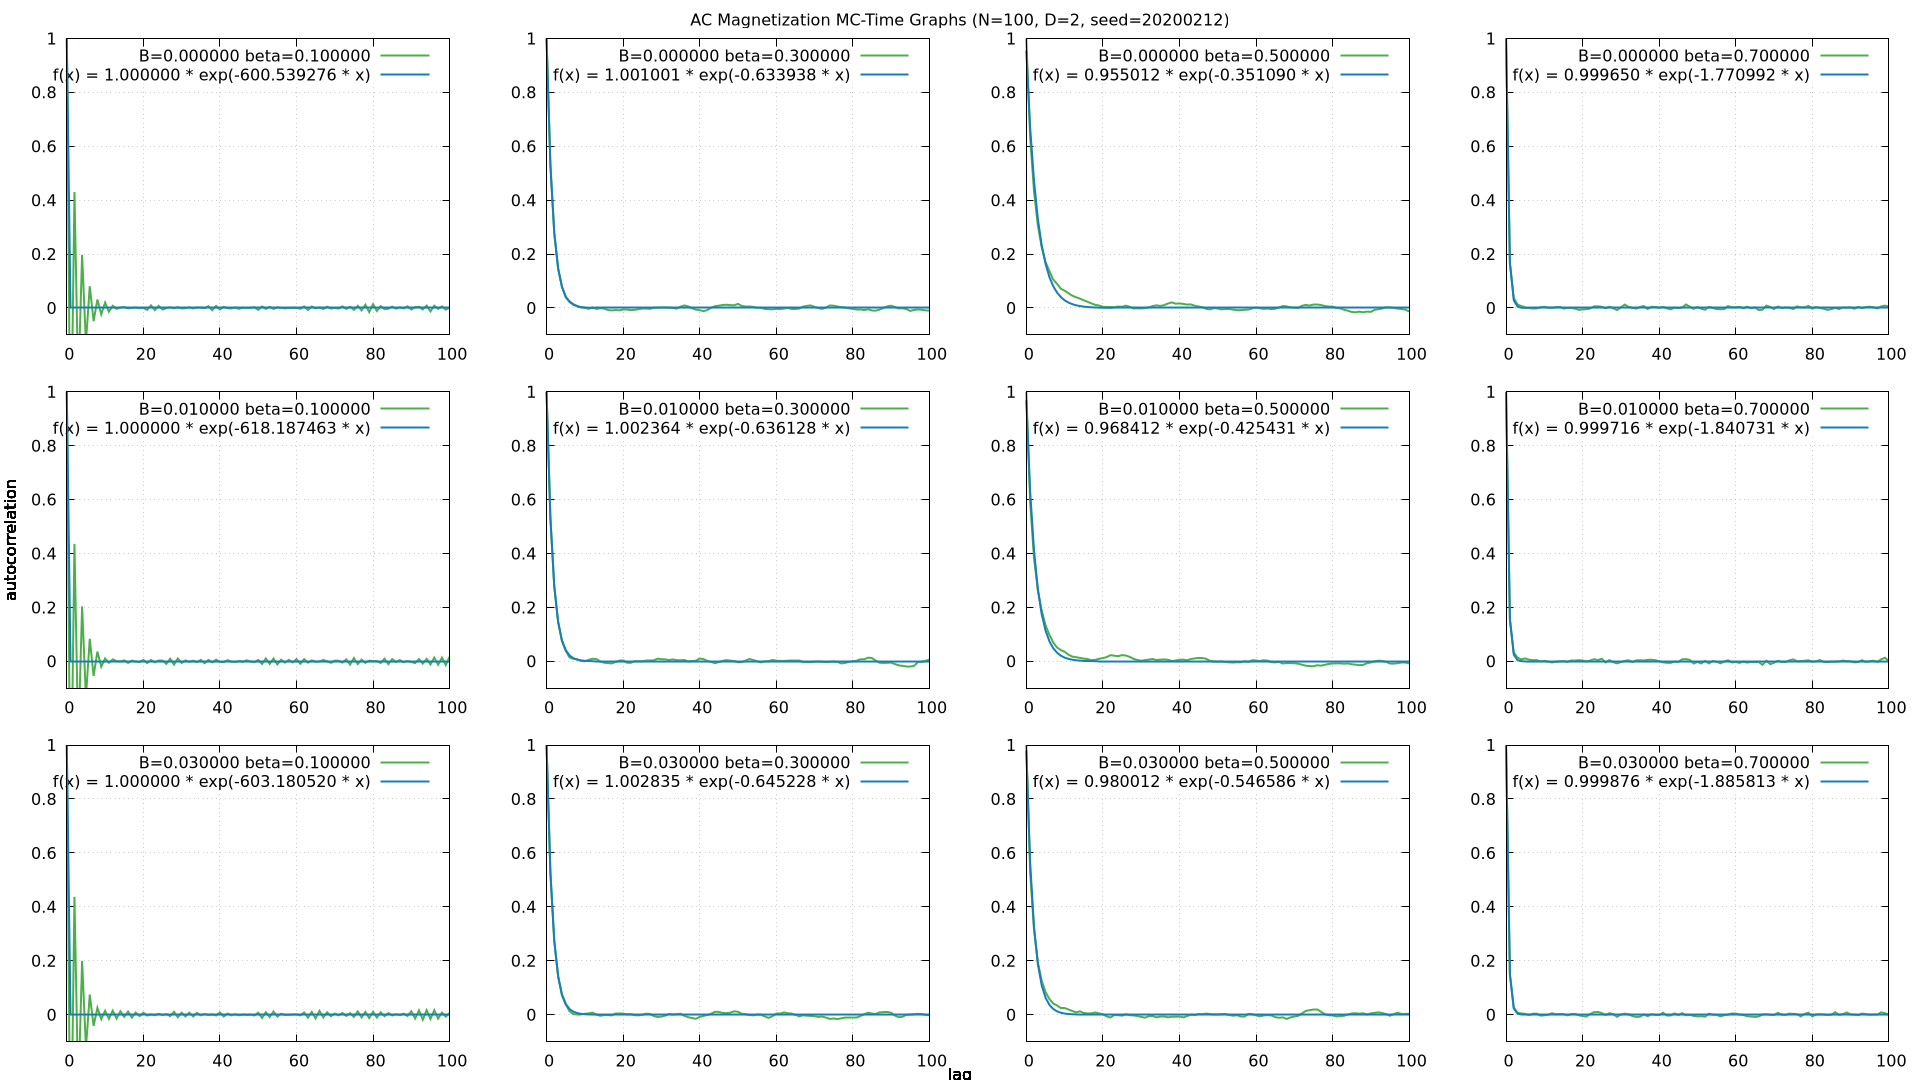
\includegraphics[scale=0.35]{all_ac_magnet.png}
\caption{Autocorrelation plotted against the mc-step using the magnetization}.
\label{fig:foo71}
\end{sidewaysfigure}

\begin{sidewaysfigure}
\centering
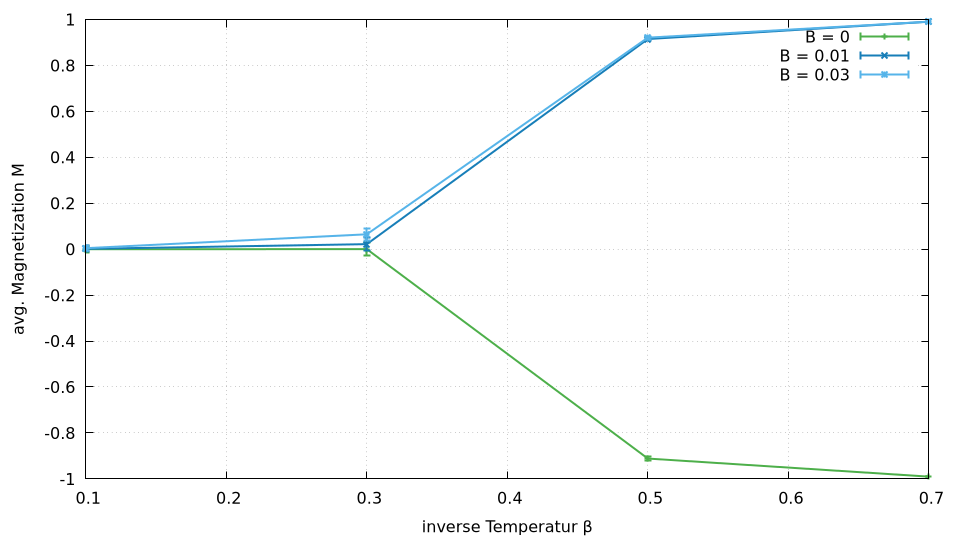
\includegraphics[scale=0.65]{magnet_beta.png}
\caption{Magnetizations as functions of $B$ and $\beta$. A clear fork form shows that at lower temperature the system starts magnetizing. For the errrorbars the standard deviation is used. Here $N = 100$ and $D = 2$.}.
\label{fig:foo70}
\end{sidewaysfigure}
\begin{sidewaysfigure}
\centering
\includegraphics[scale=0.5]{auto_corr_time.png}
\caption{Integrated autocorrelation time plotted against the lag for $B = 0.01, \beta = 0.05$. Here $N = 100$ and $D = 2$.}
\label{fig:foo70}
\end{sidewaysfigure}
\begin{sidewaysfigure}
\centering
\includegraphics[scale=0.5]{auto_correlation_function.png}
\caption{Autocorrelation function for $B = 0.01, \beta = 0.05$, $N = 100$ and $D = 2$.}
\label{fig:foo32}
\end{sidewaysfigure}


\begin{table}[]
\resizebox{\textwidth}{!}{%
\begin{tabular}{lllllllllllll}
\ B  & $\beta$ & mc-step - t & $<H>/V$        & $\sigma/V$ & t\_ac\_E & 1/t\_ac\_E & err $<H>/V$    & $<M>/V$        & $\sigma/V$ & t\_ac\_M & 1/t\_ac\_M & err/V    \\
0.00 & 0.1  & 49994      & -0.203148 & 0.014610 & 4.096215 & 0.244128   & 0.000187 & -0.000005 & 0.012492 & 0.605424 & 1.651735   & 0.000061 \\
0.00 & 0.3  & 49991      & -0.704547 & 0.017910 & 2.662914 & 0.375529   & 0.000185 & 0.000169  & 0.026975 & 2.159813 & 0.463003   & 0.000251 \\
0.00 & 0.5  & 49760      & -1.745702 & 0.017071 & 1.669934 & 0.598826   & 0.000140 & -0.911395 & 0.008823 & 2.439779 & 0.409873   & 0.000087 \\
0.00 & 0.7  & 49873      & -1.963829 & 0.005660 & 1.638106 & 0.610461   & 0.000046 & -0.990178 & 0.001656 & 1.790270 & 0.558575   & 0.000014 \\
0.01 & 0.1  & 49992      & -0.203520 & 0.014479 & 3.612930 & 0.276784   & 0.000174 & 0.001585  & 0.012588 & 0.582049 & 1.718069   & 0.000061 \\
0.01 & 0.3  & 49990      & -0.705213 & 0.017823 & 1.415181 & 0.706623   & 0.000134 & 0.022028  & 0.027060 & 1.631324 & 0.612999   & 0.000219 \\
0.01 & 0.5  & 49800      & -1.761127 & 0.016768 & 1.891486 & 0.528685   & 0.000146 & 0.914916  & 0.008170 & 2.593019 & 0.385651   & 0.000083 \\
0.01 & 0.7  & 49750      & -1.974382 & 0.005615 & 1.282258 & 0.779874   & 0.000040 & 0.990372  & 0.001631 & 1.297365 & 0.770793   & 0.000012 \\
0.03 & 0.1  & 49995      & -0.203499 & 0.014421 & 3.465091 & 0.288593   & 0.000170 & 0.004667  & 0.012541 & 0.678496 & 1.473848   & 0.000065 \\
0.03 & 0.3  & 49993      & -0.710342 & 0.018062 & 1.569072 & 0.637319   & 0.000143 & 0.064966  & 0.026734 & 2.194296 & 0.455727   & 0.000250 \\
0.03 & 0.5  & 49930      & -1.791011 & 0.016173 & 1.808575 & 0.552921   & 0.000138 & 0.920901  & 0.007277 & 2.348448 & 0.425813   & 0.000071 \\
0.03 & 0.7  & 49940      & -1.995429 & 0.005569 & 1.522384 & 0.656865   & 0.000043 & 0.990735  & 0.001597 & 1.569569 & 0.637117   & 0.000013
\end{tabular}%
}
\caption{Raw data of some parameters. Here $N = 100$ and $D = 2$.}
\label{tabel}
\end{table}


\end{document}


